\section{\scshape kNN - dodatkowe}

\subsection{Złożono"sć}
\begin{frame}{Złożono"sć obliczeniowa}
\begin{itemize}
	\item Niski koszt fazy uczenia się.
	\item Wysoki koszt klasyfikacji.
	\item $O(dn)$
\end{itemize}
\end{frame}

\begin{frame}{Wielowymiarowo"sć}
\begin{itemize}
	\item Dobra wydajno"sć dla niewielkiej liczby wymiarów.
	\item Przy wielu wymiarach wszystkie punkty są od siebie odległe.
	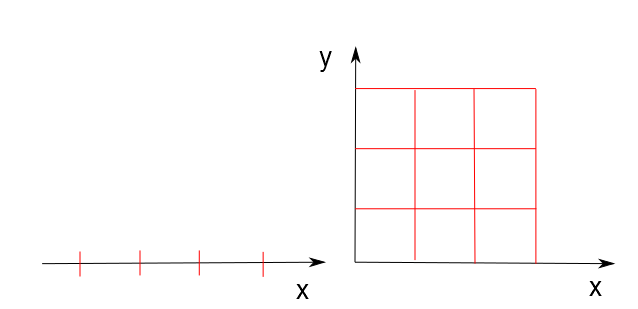
\includegraphics[keepaspectratio=true, scale=0.55]{dims_small}
\end{itemize}
\end{frame}


\subsection{Ważone kNN}
\begin{frame}{Ważone kNN}
\begin{itemize}
	\item Sąsiedzi położeni blisko mają większą wagę
	\item \textbf{Każdy} sąsiad bierze udział w etykietowaniu.
	\item Decyduje ważona większo"sć.
\end{itemize}
\end{frame}


\subsection{Zastosowanie}
\begin{frame}{Zastosowanie}
\begin{itemize}
	\item Sytuacje trudne do modelowania w klasyczny sposób.
	\item Zależno"sć między zmiennymi jest nietypowa.
	\item Metody klasyczne są bardziej użyteczne w przypadku niezłożono"sci relacji.
\end{itemize}
\end{frame}